\section{Analysis}

To aid the analysis, we assume that the ITIs contain all the previous transcript
of their execution (a history of machine configurations).

% \begin{definition}[Determinism]
%       Let $\Pi^\Sigma$ be a State Machine Replication protocol that makes
%       oracle use of a signature protocol $\Sigma = (\textsf{Gen}, \textsf{Sig}, \textsf{Ver})$.
%       The protocol $\Pi$ is called \emph{soft deterministic} if,
%       when executed as an interactive turing machine $\Pi^\Sigma(i)$ initialized for party
%       with index $i$, the machine does not make use of any local randomness.
% \end{definition}
%
% TODO: define underlying, overlay, good, VIEW...

% TODO: Move this to definitions? Expand this intuitive explanation,
% and give it a title
% Potential generalization: Use a different H_Z and H_Y that indicate
% which Ys are "good" and which Zs are supposed to be "honest", and
% make H_Z a function of H_Y, to be defined by the DPCP.
% This would allow having a different number of Zs and Ys,
% and each of the Zs could depend on different, and potentially multiple, Ys;
% and each Y could help multiple Zs.

A \emph{compositor} is a protocol that
runs an \emph{overlay} distributed protocol $\Pi$ on top of a set of
$n$ \emph{underlying} distributed protocols $\Y[][1], \ldots, \Y[][i], \ldots, \Y[][n]$.
The protocol $\Pi$ is generally designed
to work in the \emph{party setting} with a network (such as an authenticated channels network)
connecting its instances directly.
The compositor $\Lambda$ executes
$\Pi$ in the \emph{emulated setting} by utilizing the underlying
$\Y[][i]$ protocols to help with the emulation and communication between the
overlay protocol instances.
Multiple instances $\LLambda[1], \ldots, \LLambda[j], \ldots, \LLambda[m]$
of the compositor are executed.
Each $j^\text{th}$ compositor instance promises to emulate the execution of multiple
instances of $\Pi$ ($\Z[j][1], \ldots, \Z[j][i], \ldots \Z[j][n]$).
These emulated $\Z$ instances should behave similarly to instances of $\Pi$
running in a stand-alone setting.

\begin{definition}[Compositor]
  A \emph{compositor} $\Lambda$ with overlay $\Pi$ and underlying $\mathcal{Y} = \Y[][1], \ldots, \Y[][n]$,
  is a family of interactive machines
  $\Lambda_{\Pi,\mathcal{Y}}$ providing the following
  functionalities:

  \begin{enumerate}
    \item \construct$(\sid, (\Y[j][1] \ldots \Y[j][n]))$.
    \item \writeToMachine$(i, \data)$.
    \item \emulateMachine$(i, r)$. % <-- Z
  \end{enumerate}
\end{definition}

The compositor is constructed by calling \emph{\construct} with parameter the session identifier $\sid$.
Note that compositors are permissionless, as they don't know their instance identity $j \in \mathbb{N}$.
Each compositor instance provides a \emph{\writeToMachine}
functionality that allows writing data to the $i^\text{th}$ emulated machine.
It also provides an \emph{\emulateMachine} functionality that promises to emulate the execution of
the $i^\text{th}$ instance of $\Pi$ up to round $r$, and return the instance of this emulation
at round $r$ (and note that this contains the full transcript of the emulation).
Observe that \emph{\emulateMachine} can be invoked at a later round $r' > r$.
Note here the difference between $\mathcal{Y} = \Y[][1], \ldots, \Y[][n]$ (denoting \emph{underlying protocols}
in the form of ITMs) and
$(\Y[j][1], \ldots, \Y[j][n])$ (denoting \emph{underlying protocol instances}
in the form of ITIs). The compositor is parametrized with the former, and
the latter are passed as parameters to the \emph{\construct} functionality.

Even though we will not do the analysis in the full Universal Composability (UC) framework, and
we treat executions as stand-alone, we do adopt some of the notation of the UC framework.
Let $\LCExec(\Lambda, \mathcal{Y}, \mathcal{A}, \mathcal{Z})$
denote the transcript of an execution of the compositor protocol $\Lambda$ parametrized with overlay protocol $\Pi$,
and underlying protocols $\mathcal{Y} = (\Y[][1], \ldots, \Y[][n])$, adversary $\mathcal{A}$, and environment $\mathcal{Z}$.
Following the notation of the UC framework, we define the notion of an \emph{execution}
and a \emph{view}.

\noindent
\textbf{The Emulated Setting.}
In particular, in the emulated setting execution, denoted by $\LCExec_{m,n}(\Lambda, \mathcal{Y}, \mathcal{A}, \mathcal{Z})$,
the environment $\mathcal{Z}$ is constrained by the control program
to initially
spawn a number $n \times \ell$ (where $n$ is a parameter of the execution,
and $\ell = |\mathcal{Y}|$)
underlying protocol instances

\begin{align*}
\Y[1][1], \Y[1][2], &\ldots, \Y[1][\ell],\\
\Y[2][1], \Y[2][2], &\ldots, \Y[2][\ell],\\
                    &\vdots              \\
\Y[m][1], \Y[m][2], &\ldots, \Y[m][\ell]\,,
\end{align*}

where $\Y[j][i]$ denotes the $j^\text{th}$ instance of
the protocol $\Y[][i]$. The environment facilitates the communication
between the underlying protocol instances $\Y[j][i]$ and $\Y[j'][i]$
for all $j, j'$, whereas protocols $\Y[j][i]$ and $\Y[j'][i']$
with $i \neq i'$ are not allowed to directly communicate.
Next, the environment is constrained to spawn
a number $m$ of compositor clients
$\LLambda[1], \ldots, \LLambda[m]$ (where $m \in \mathbb{N}$
is a parameter of the execution), allowing
the environment to choose the $\sid$ parameter,
and passing the tuple $(\Y[j][1], \ldots, \Y[j][\ell])$ of ITIs
to $\LLambda[j]$'s \emph{construct} functionality
(in UC language, each of these $\Y[j][i]$ is constrained to be used
as a \emph{subroutine} solely by $\LLambda[j]$).
All of those $\Lambda$ compositor clients are honest and will remain
so throughout the execution.
Outside of those $\Y[j][i]$ instances controlled by the $\Lambda$s, each of
the protocols $\Y[][i]$ may have more instances running within the execution,
spawned by the environment and potentially corrupted by the adversary.
For example, if $\Y[][1]$ is the Bitcoin protocol, then the $\Y[j][i]$
instance running within $\LLambda[j]$ is a Bitcoin client, whereas the
execution comprises also others Bitcoin clients and full nodes, potentially
corrupted by the adversary.
The execution proceeds in rounds $r = 1, \ldots, R$
for a polynomial number $R$ of rounds (where the polynomial
is taken with respect to the security parameter). For every
round $r$, the environment is constrained to first call
the \emph{execute} function of each $\Y[j][i]$ for every
$j, i \in \mathbb{N}$, as well as the \emph{execute} function of $\Y$s
living outside of the clients $\Lambda$. Next, the environment must call
the \emph{execute} function of each $\LLambda[j]$ sequentially.
Finally, the environment is constrained to call the
adversary $\mathcal{Z}$ (a rushing adversary).
The adversary is allowed to corrupt the $\Y$ instances living outside of $\Lambda$s
% TODO: Can there even be a safety-respecting environment, e.g., in Streamlet or Bitcoin?
% I think the environment can only be things like honest-majority-respecting.
% How can an environment constraint the execution to be safe?
(we will later impose constraints, in the form of \emph{beliefs}, which the
environment ensures the adversary must respect).
At any time, the environment may choose to provide inputs
to any of the $\LLambda[j]$ parties by invoking their \emph{writeToMachine}
functionality with inputs of its choice.

\noindent
\textbf{The Party Setting.}
In the party setting execution, denoted by $\PEExec_n(\Pi,\allowbreak \mathcal{A},\allowbreak \mathcal{Z},\allowbreak n,\allowbreak H,\allowbreak \Delta)$,
the environment $\mathcal{Z}$ is constrained by the control program
to spawn $n$ parties $\PPi[1], \ldots, \PPi[n]$ (where $n \in \mathbb{N}$
is a parameter of the execution). Note here that $\Pi$ is a protocol (an ITM),
whereas each $\PPi[i]$ is an instance (an ITI).
The adversary $\mathcal{A}$ is allowed to corrupt parties
indexed by $[n] \setminus H$ at the beginning of the execution
(a static corruption model). This is done by the adversary sending a message
to the environment requesting to corrupt the desired party. The environment
grants this corruption wish as long as it respects the requirement that the
corruption falls within $[n] \setminus H$.
The execution proceeds in rounds
$r = 1, \ldots, R$, where $R$, again, is a polynomial of the security
parameter. At every round, the environment is constrained to first
call the \emph{execute} function of each $\PPi[i]$ for every
honest party, in order. Next, the environment must call
the adversary (again, a rushing adversary). The environment
is constrained to deliver messages between honest parties
in an authenticated manner, and to deliver messages within $\Delta$
delay.

We would like to define a notion of \emph{faithfulness} of a
compositor, which captures the
correspondence between the party setting execution and the emulated setting
execution of $\Pi$. Roughly, a compositor is called \emph{faithful} is these
two settings are identical in the eyes of the honest parties.
This faithfulness may be conditioned to work only on certain classes
of overlay protocols $\Pi$ and underlying protocols $\Y$, and may
require that a certain subset $\mathcal{H}$ of these $\Y$s are well-behaved.

\begin{definition}[Compositor Faithfulness (informal)]
We say that a compositor $\Lambda$ is \emph{faithful} for an overlay protocol $\Pi$,
a number of overlay parties $n \in \mathbb{N}$ running
over a number of underlying protocols $\mathcal{Y} = (\Y[][1], \ldots, \Y[][\ell])$
if:
For all number of compositor parties $m \in \mathbb{N}$,
for every compositor index $j \in [m]$,
for every overlay index $i \in [n]$ that ``corresponds' to ``well-behaving'' underlying $\mathcal{Y}$s
it holds that:
The party $\Z[j][i]$'s emulated execution ``is identical'' to \emph{some} party setting execution
(it cannot tell if it is emulated or not).
Within that emulated execution, the emulated instance $\Z[j][i]$
is given the ``same'' inputs as \emph{write}(\emph{data}) by its environment
as the compositor is given by its own environment as \emph{writeToMachine}(i, \emph{data})
for that same $i$.
\end{definition}

The motivation for the above definition stems from the fact that, if it is known that
$\Pi$ is secure in the party setting, these security results can be translated to the
emulated setting. The full definition of faithfulness will state that for all adversaries
in the emulated setting, there is a simulator in the party setting that makes the
views of honest parties identical. Since the protocol $\Pi$ is secure in the party setting
under that simulator, it must also be secure in the emulated setting under any adversary.
This line of argument is not unlike Canetti's UC arguments.

While the fact that the view of the honest party is the same in both the emulated and
party setting is sufficient to argue that the \emph{write} instructions in both settings will
be the same in the views of the honest parties, this will not be sufficient.
The last part of the definition sketch above whereby the \emph{writeToMachine} instructions
of the emulated setting are replicated as \emph{write} instructions in the party setting
is a necessary ingredient to make the definition useful. Otherwise, trivial constructions
in which \emph{writeToMachine} instructions are ignored are possible, yet we want to avoid
such pathologies.

To make the above definition precise, we must develop a number of tools. Namely,
we must state what ``well-behaving'' underlying protocols are, and what the ``correspondence''
between overlay parties and underlying protocols means. Furthermore, we must specify
what the ``identical'' emulated execution means, and what the ``same'' inputs are,
in which definitions we will be required to allow for some slack.

We define the following views for the two execution settings.

\begin{definition}[Honest View in the Party Setting]
  Consider a party setting execution $\mathcal{E}'$ of duration $R$ rounds
  sampled from
  $\PEExec_n(\Pi,\allowbreak \mathcal{A},\allowbreak \mathcal{Z},\allowbreak n,\allowbreak H,\allowbreak \Delta)$.
  The \emph{party setting view of honest parties} $\PEView_H(\mathcal{E}')$
  is the $|H|\times R$ matrix of the following transcripts of honest parties:

  \[
  \begin{bmatrix}
    \PPi[H_1]_1 &\ldots& \PPi[H_1]_R\\
         \vdots &\ddots& \vdots     \\
    \PPi[H_{|H|}]_1 &\ldots& \PPi[H_{|H|}]_R
  \end{bmatrix}\,,
  \]

  where $\PPi[H_i]_r$ denotes the transcript of party $\PPi[H_i]$
  (the party with index $H_i$, the $i^\text{th}$ honest party)
  obtained at the end of round $r$.
\end{definition}

Note that, in the above definition, the transcripts concerned pertain to the
set $H$ of guaranteed honest party indices only, even though the adversary may choose
to leave some of the other parties uncorrupted, too. The transcript of
those other parties are not included in $\PEView_H(\mathcal{E}')$.

Note also that, in each row of the above definition, the transcripts
are taken for a particular party $H_i$ at increasing rounds, and therefore
we will have that $\PPi[H_i]_r \preceq \PPi[H_i]_{r+1}$ and, so, the transcripts
recorded in each row will be growing in an append-only fashion.

\begin{definition}[Emulation Consistency]
  An execution $\mathcal{E}$ with duration $R$ rounds sampled from
  $\LCExec_m(\Lambda, \mathcal{Y}, \mathcal{A}, \mathcal{Z})$
  is \emph{$(j,H,\Delta_v)$-\emph{consistent}},
  for a compositor index $j \in [m]$,
  a set of overlay machine indices $H \subseteq [n]$,
  and reality lag $\Delta_v$,
  if
  for all $i \in H$, for all $r \geq 0$,
  for all $r + \Delta_v < r' < R$,
  it holds that
  $\LLambda[j].\emulateMachine(i, r)$ executed \emph{in vitro} at the end of round $r'$
  is equal to
  $\LLambda[j].\emulateMachine(i, r)$ executed \emph{in vitro} at the end of round $r' + 1$.
\end{definition}

Note that in the above definition, we allow $r = 0$, even though rounds
in the execution begin at $1$.

\begin{definition}[Honest View in the Emulated Setting]
  Consider an emulated setting execution $\mathcal{E}$ with duration $R$ rounds
  sampled from $\LCExec_m(\Lambda, \mathcal{Y}, \mathcal{A}, \mathcal{Z})$.
  If the execution $\mathcal{E}$ is $(j,H,\Delta_v)$-consistent, then
  the \emph{emulated setting view of honest parties} $\LCView_{j,H,\Delta_v}(\mathcal{E})$,
  % TODO: change "reality lag" to be a generic "time distortion" function,
  % for now f(r) = r + \Delta_v, but this could be more generic
  parametrized by an index $j$, a set of indices $H$, and a \emph{reality lag} $\Delta_v \in \mathbb{N}$,
  is the $|H| \times R$ matrix of the following values:

  \[
  \begin{bmatrix}
    \LLambda[j].\emulateMachine(H_1, 1) & \ldots & \LLambda[j].\emulateMachine(H_1, R - \Delta_v - 1)\\
                                 \vdots & \ddots & \vdots \\
    \LLambda[j].\emulateMachine(H_{|H|}, 1) & \ldots & \LLambda[j].\emulateMachine(H_{|H|}, R - \Delta_v - 1)
  \end{bmatrix}\,,
  \]

  where $\LLambda[j].\emulateMachine(H_i, r)$ denotes the return value of invoking,
  \emph{in vitro} at the end of round $r + \Delta_v + 1$,
  the $\emulateMachine$ functionality of the $j^\text{th}$ compositor party $\LLambda[j]$
  with parameters the index $H_i$ of the $i^\text{th}$ overlay machine (among those
  included in $H$) and round $r$.

  On the other hand, if the execution $\mathcal{E}$ is \emph{not} $(j,H,\Delta_v)$-consistent, then
  we let $\LCView_{j,H,\Delta_v}(\mathcal{E}) = \bot$.
\end{definition}

\begin{definition}[Party Setting Externalities]
  Consider a party setting view $V$ of honest parties and size $|H| \times R$.
  The \emph{party setting externalities} $\PEExtern(V)$ is the $|H| \times R$ matrix:
  \[
  \begin{bmatrix}
    \W[H_1][1] &\ldots& \W[H_1][R]\\
         \vdots &\ddots& \vdots     \\
    \W[H_{|H|}][1] &\ldots& \W[H_{|H|}][R]
  \end{bmatrix}\,,
  \]

  where $\W[H_i][r]$ denotes the sequence of messages written into an honest party
  with index $H_i$ during round $r$. This sequence of messages can be extracted from
  the transcript $\PPi[H_i]_r$ found in $V$.
\end{definition}

\begin{definition}[Emulated Setting Externalities]
  Consider an emulated setting execution $\mathcal{E}$ with duration $R$ rounds
  sampled from $\LCExec_m(\Lambda,\allowbreak \mathcal{Y},\allowbreak \mathcal{A},\allowbreak \mathcal{Z})$.
  Consider the transcript of compositor client $\LLambda[j]$ in $\mathcal{E}$.
  Within that transcript, observe the \emph{writeToMachine} calls made by
  $\mathcal{Z}$ on $\LLambda[j]$ during some fixed round $1 \leq r \leq R$.
  Among those, consider the calls to \emph{writeToMachine} that were
  invoked with first argument some fixed machine index $1 \leq i \leq m$.
  These \emph{writeToMachine} calls were invoked, in order, as
  $\writeToMachine(i, \data_1), \ldots, \writeToMachine(i, \data_k)$
  all during round $r$.
  Let $\W[i][r] = (\data_1,\allowbreak\ldots,\allowbreak\data_k)$ denote the sequence containing
  all the \emph{data} parameter values of those calls.
  The \emph{emulated setting externalities} $\LCExtern_{j,H}(\mathcal{E})$, parametrized
  by an index $j$ and a set of indices $H$, is the $|H| \times R$ matrix:

  \[
  \begin{bmatrix}
    \W[H_1][1] &\ldots& \W[H_1][R]\\
         \vdots &\ddots& \vdots     \\
    \W[H_{|H|}][1] &\ldots& \W[H_{|H|}][R]
  \end{bmatrix}\,.
  \]
\end{definition}

\begin{definition}[Externality Similarity]
  Consider the externalities $E_1, E_2$ (in the party or emulated setting)
  with dimensions $n \times R_1$ and $n \times R_2$ respectively.
  We say that $E_1$ is \emph{similar} to $E_2$ with \emph{lateness} parameter
  $\Delta_u \in \mathbb{N}$ and \emph{earliness} parameter $\Delta_v \in \mathbb{N}$, written
  $E_1 \laterly{\Delta_u,\Delta_v} E_2$, if
  the following holds:
  For any message $m$ located within the writebox at position $(i, r)$ of $E_1$,
  with $r < R_1 - \Delta_u - \Delta_v$,
  there exists a round $r - \Delta_v \leq r' \leq r + \Delta_u$ such that
  the message $m$ appears within the writebox at position $(i, r')$ of $E_2$.

  Furthermore, we say that the random variable $E_1$
  is \emph{distributionally similar} to $E_2$
  with \emph{lateness} parameter $\Delta_u \in \mathbb{N}$
  and \emph{earliness} parameter $\Delta_v \in \mathbb{N}$,
  written $E_1 \laterlydistr{\Delta_u,\Delta_v} E_2$, if
  there is a mapping $f: \supp(E_1) \rightarrow \supp(E_2)$
  such that for all $x \in \supp(E_1)$, $x \laterly{\Delta_u,\Delta_v} f(x)$ and
  for all $y \in \supp(E_2)$, $\Pr[E_2 = y] = \sum_{x \in f^{-1}(y)} \Pr[E_1 = x]$.
\end{definition}


\begin{definition}[Belief]
  A \emph{belief} $B$ is any predicate over an execution $\mathcal{E}$.
\end{definition}

For example, given an execution $\mathcal{E}$, with underlying distributed ledger
protocols $\mathcal{Y} = (\Y[][1], \ldots, \Y[][\ell])$, we can define a belief
$B$ asserting that the majority of underlying ledger protocols are secure.

\begin{definition}[Belief System]
  A \emph{belief system} $\mathcal{B}$ is a set of beliefs.
\end{definition}

\begin{definition}[Honesty Correspondence]
  Given a belief system $\mathcal{B}$ and a number $n \in \mathbb{N}$ of overlay parties,
  an \emph{honesty correspondence} $\mathcal{H}(B)$ is any function
  from $\mathcal{B} \longrightarrow 2^{[n]}$.
\end{definition}

\begin{definition}[Belief-Respecting Environment]
  An environment $\mathcal{Z}$ is \emph{belief-respecting} for a belief $B$
  if for all executions $\mathcal{E}$ in the support of
  a given distribution of executions, it holds that $B(\mathcal{E})$.
\end{definition}

% TODO: Mention that the validator and other protocol settings for \Y[][i]
% are hard-coded into \Y[][i]
\begin{definition}[Compositor Faithfulness]\label{def:faithfulness}
  A compositor $\Lambda$
  is $(\Pi,\allowbreak n,\allowbreak \mathcal{Y},\allowbreak \mathcal{B},\allowbreak \mathcal{H},\allowbreak \Delta_u,\allowbreak \Delta_v)$-\emph{faithful}
  for an overlay protocol $\Pi$,
  a number of overlay parties $n \in \mathbb{N}$,
  a sequence of underlying protocols $\mathcal{Y} = (\Y[][1], \ldots, \Y[][\ell])$,
  a belief system $\mathcal{B}$,
  honesty correspondence $\mathcal{H}: \mathcal{B} \longrightarrow 2^{[n]}$,
  lateness $\Delta_u \in \mathbb{N}$,
  and reality lag $\Delta_v \in \mathbb{N}$
  if:

  For all beliefs $B \in \mathcal{B}$,
  for all PPT adversaries $\mathcal{A}$ and all
  $B$-respecting PPT environments $\mathcal{Z}$,
  for all number of compositor parties $m \in \mathbb{N}$,
  for all compositor party indices $j \in [m]$,
  % TODO: There is no need for the polynomiality constraint on A and Z,
  % but the reduction maintains polynomiality
  there is a PPT simulator $\mathcal{S}$ and there is a
  PPT environment $\mathcal{Z}'$ such that
  the following holds:

  \begin{enumerate}
    \item $\LCView_{j,\mathcal{H}(B),\Delta_v}(\mathcal{E}) \distreq \PEView_{\mathcal{H}(B)}(\mathcal{E}')$
    \item $\LCExtern_{j,\mathcal{H}(B)}(\mathcal{E}) \laterlydistr{\Delta_u,\Delta_v} \PEExtern(\PEView_{\mathcal{H}(B)}(\mathcal{E}'))$
  \end{enumerate}

  where execution $\mathcal{E}$ is sampled from
  % TODO: Do not use "EXEC", as this is inconsistent with the UC framework
  $\LCExec_m(\Lambda, \mathcal{Y}, \mathcal{A}, \mathcal{Z})$
  % TODO: B should only depend on the collective execution of \Y, not anything else
  and execution $\mathcal{E}'$ is sampled from
  $\PEExec(\Pi, \mathcal{S}, \mathcal{Z}', n, \mathcal{H}(B), \Delta)$,
  and $\Delta = \Delta_v + \Delta_u$.
\end{definition}

% Remark: Differences from a UC-style proof

\begin{lemma}[Past Perfect]\label{lem:past-perfect}
  Consider a temporal ledger protocol $\Y$'s
  execution $\Exec$ with duration $R$ rounds in which $\Y$ is
  safe, live with liveness $u$, and timely with timeliness $v$.
  If for some honest party $P_1$ and some round $r_1$ it holds that
  $(r^*, \tx) \in \Ledger[P_1][][r_1]$, then
  for all honest parties $P_2$ and for all rounds $r_2 > r^* + v$
  it holds that
  $(r^*, \tx) \in \Ledger[P_2][][r_2]$,
  % TODO:
  % We may be able to remove this extra assumption if
  % we change temporal ledgers to also report their "current time"
  % under the following constraints:
  % 1) In synchronous settings, or after GST in psync, the "current time"
  %    reported by the ledger must not be too far in the past (more than $v$?)
  % 2) The "current time" reported must march only forward;
  %    the next "current time" reported must be larger than the
  %    current "current time" reported.
  % 3) If I read the ledger at some round r_1 and the current time reported
  %    is r_1', then I read the ledger again at round r_2 > r_1, then
  %    any *new* transactions that appear must have a recorded round of
  %    at least r_1'.
  % We may be able to replace "timeliness" completely with the above
  % definition.
  as long as at least one new honest transaction $\tx'$ appears at
  any round $r_1 < r_3 \leq R - u$.
\end{lemma}
\begin{proof}
  Consider an execution as in the statement and suppose, towards a contradiction,
  that $(r^*, \tx) = \Ledger[P_1][][r_1][k]$ for some $k \in \mathbb{N}$,
  but $(r^*, \tx) \not\in \Ledger[P_2][][r_2]$
  with $r^* + v < r_2$.
  From safety,
  $\Ledger[P_2][][r_2] \prec \Ledger[P_1][][r_1]$ and
  $|\Ledger[P_2][][r_2]| \leq k < |\Ledger[P_1][][r_1]|$.
  Due to liveness, $(r', \tx') = \Ledger[P_2][][r_3 + u][k']$,
  for some $r', k' \in \mathbb{N}$.
  As $\tx'$ is new, it is not in $\Ledger[P_1][][r_1]$.
  Due to safety, $k' \geq |\Ledger[P_1][][r_1]| > k$.
  Due to safety, $\Ledger[P_2][][r_3 + u][k] = (r^*, \tx)$.
  Therefore
  $(r^*, \tx) \in \Ledger[P_2][][r_3 + u][|\Ledger[P_2][][r_2]|{:}]$.
  Since $r^* < r_2 - v$, this contradicts the timeliness with parameter $v$.\qed
\end{proof}

The above property, which follows from safety, liveness, timeliness and
contiguous honest participation is also known in the literature as
\emph{persistence}~\cite{backbone}.

\begin{definition}[Rollerblade Belief System and Honesty Correspondence]
  Given a sequence of \rollerblade-underlying-respecting
  protocols $\mathcal{Y} = (\Y[][1], \ldots, \Y[][\ell])$,
  define for each $i \in [\ell]$ the following predicate on
  a collective execution $\mathcal{E}$ of $\mathcal{Y}$:

  \[
    \text{good}_i(\mathcal{E}) = \text{``} \Y[][i] \text{ is safe, live$(u_i)$, and timely$(v_i)$ in $\mathcal{E}$''}
  \]

  Next, for any $H \subseteq [\ell]$, we define:

  \[
    \text{good}_H(\mathcal{E}) = \text{``}\forall i \in H: \text{good}_i(\mathcal{E})\text{''}
  \]

  Define $\mathcal{H}^{-1}$ on the domain $2^{[n]}$ as
  $\mathcal{H}^{-1}(H) = \text{good}_H$.
  Then the \emph{\rollerblade honesty correspondence $\mathcal{H}$}
  is the inverse of $\mathcal{H}^{-1}$ and the \emph{\rollerblade belief system
  $\mathcal{B}$} is the domain of $\mathcal{H}$.
\end{definition}

For example, if $\mathcal{Y} = (\Y[][1], \Y[][2], \Y[][3])$,
then for $B = \text{good}_1 \land \text{good}_3$, it holds that
$B \in \mathcal{B}$ and $\mathcal{H}(B) = \{1, 3\}$.

As an example of a $\Y[][1]$, consider the Bitcoin Backbone protocol.
Then a $\text{good}_1$-respecting environment $\mathcal{Z}$ is an environment
that ensures the Bitcoin Backbone protocol execution is safe, live, and timely.
This can be done, for example, by demanding that the corruption of $\Y[][1]$
parties outside of $\Lambda$s remains in the minority. In case the environment
detects an upcoming security violation (due to a negligible event such as a
Random Oracle collision), it can conclude the execution.

\begin{lemma}[Rollerblade Cross-party]\label{lem:cross-party}
  Consider a \rollerblade execution $\mathcal{E}$ with duration $R$ rounds
  with $n \in \mathbb{N}$ underlying
  and $m \in \mathbb{N}$ compositor parties.
  For
  all underlying indexes $i \in [n]$ such that $\text{good}_i(\mathcal{E})$,
  all rounds $1 \leq r < R - \max(v_i, u_i)$,
  and
  all compositor party indexes $j, j' \in [m]$

  \[
    \Sim[j][r] = \Sim[j'][r]\,,
  \]

  where $\Sim[j][r]$ (resp. $\Sim[j'][r]$) indicates the result of calling
  \emulateMachine of $\RB[j]$ (resp. $\RB[j']$) with inputs
  $(i, r)$
  \emph{in vitro} at the end of round $r + v_i$ of $\mathcal{E}$.
\end{lemma}
\begin{proof}
  The function \emulateMachine of party $j$ (resp. party $j'$)
  calls the deterministic function \simulate with overlay party index $i$,
  ledger $\Ledger[j][i][r + v_i]$ (resp. ledger $\Ledger[j'][i][r + v_i]$), simulation round
  $r$, and current round $r + v_i$. The function \simulate runs its main
  \emph{for} loop (Algorithm~\ref{alg.simulate} Line~\ref{alg.simulate:for})
  up to $r$ (inclusive), which consumes data from $\writeboxes[r - 1]$
  and $\inboxes[r - 1]$ and earlier. These are produced by the function
  \prepareSimulationInputs by looking at transactions recorded in $\Ledger[j][i][r + v_i]$
  (resp. $\Ledger[j'][i][r + v_i]$) with recorded round $< r$.
  Because $\Ledger[][i]$ is \emph{good} in $\mathcal{E}$, it is safe, live($u_i$), and timely($v_i$).
  It suffices to show that all transactions with recorded round
  $< r$ are the same in $\Ledger[j][i][r + v_i]$ and $\Ledger[j'][i][r + v_i]$.
  This holds because of Lemma~\ref{lem:past-perfect} invoked with parties $\Y[j][i]$ and $\Y[j'][i]$,
  rounds $r_1 = r_2 = r + v_i$, $r_3 = r + v_i + 1$ and $r^* < r$.
  During round $r_3$, the new honest transaction is due to any honest
  relayer.\qed
\end{proof}

\begin{figure*}
  \centering
  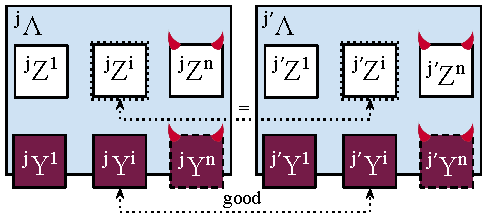
\includegraphics[width=0.6 \textwidth,keepaspectratio]{figures/rollerblade-cross-party.pdf}
  \caption{The Cross-Party Lemma (Lemma~\ref{lem:cross-party}) states that
  the execution of the emulated machines $\Z[j][i]$ and $\Z[j'][i]$
  across two different compositor parties $\LLambda[j]$ and $\LLambda[j']$
  is consistent, as long as the underlying ledger $\Y[][i]$ is \emph{good}.}
  \label{fig.cross-party}
\end{figure*}

\begin{lemma}[Rollerblade Consistency]\label{lem:consistency}
  Consider a \rollerblade $\Lambda$ execution $\mathcal{E}$ with duration $R$ rounds
  sampled from $\LCExec_m(\Lambda, \mathcal{Y}, \mathcal{A}, \mathcal{Z})$
  with overlay protocols $\mathcal{Y}$, adversary $\mathcal{A}$ and environment $\mathcal{Z}$,
  and let $\Delta_v = \max\{v_i\}_{i \in [n]}$,
  where $v_i$ denotes the timeliness
  promised by ledger protocol $\Y[i]$.
  Let $H \subseteq [n]$ be the subset of good underlying ledger protocol indices among $\mathcal{Y}$
  in $\mathcal{E}$.
  Then the execution is $(j, H, \Delta_v)$-consistent for all $j \in [m]$.
\end{lemma}
\begin{proof}
  Let $i \in H$, $r \geq 0$, $r + \Delta_v < r' < R$ be arbitrary.
  When $\emulateMachine$ is invoked at the end of round $r'$ (resp. $r' + 1$),
  the value $\this.\now$
  is $r'$ (resp. $r' + 1$), so the check $\simulationRound > \this.\now - v_i$ of Algorithm~\ref{alg.prepare-simulation-inputs}
  Line~\ref{alg.prepare-simulation-inputs:reality-lag} is \emph{false}, and the emulation
  succeeds. This is the only stateful check in this function.
  The result of the function $\prepareSimulationInputs$ only depends on the transactions of
  its $\Ledger[j][i]$ argument with recorded rounds up to $\simulationRound$.
  Therefore it suffices to show that the transactions in
  $\Ledger[j][i][r']$ with recorded rounds up to $\simulationRound$ are the same
  as the transactions in $\Ledger[j][i][r' + 1]$ with recorded rounds up to $\simulationRound$.
  All $\Ledger[j][i][r']$ transactions with recorded rounds up to $\simulationRound$
  are included in $\Ledger[j][i][r' + 1]$ by \emph{stickiness}.
  Conversely, all $\Ledger[j][i][r' + 1]$ transactions with recorded rounds up to $\simulationRound$
  are included in $\Ledger[j][i][r']$ by \emph{timeliness}.\qed
\end{proof}

% TODO: Consider removing all "in vitro" invocations by requiring the
% compositor to output a configuration during every round by itself within
% the execution. This would simplify the language.

% TODO: Define the relationship between Z and Z';
%       we are hoping that Z' will have exactly the same writes as Z
%       (perhaps more due to adversarial writes) for each party
%       and that those will appear in "close enough" times (maybe up to $u$ away
%       from the original)
\begin{conjecture}[Rollerblade Simulation]\label{conj:simulation}
  For all \rollerblade-suitable-overlay protocols $\Pi$
  and any sequence of \rollerblade-suitable-underlying
  protocols $\mathcal{Y} = (\Y[][1], \ldots, \Y[][\ell])$
  for the \rollerblade-belief-system $\mathcal{B}$ of $\mathcal{Y}$
  and honesty correspondence $\mathcal{H}$,
  the compositor \rollerblade of Section~\ref{sec:construction} is
  $(\Pi, n, \mathcal{Y}, \mathcal{B}, \mathcal{H}, \Delta_u, \Delta_v)$-\emph{faithful},
  where $n = \ell$, $\Delta_u = \max\{u_i\}_{i \in [n]}$,
  $\Delta_v = \max\{v_i\}_{v \in [n]}$
  and $u_i, v_i$ are the promised liveness and timeliness of $\Y[][i]$.
\end{conjecture}
\begin{proof}[Sketch]
  Let $\Pi$, $\mathcal{Y}$, $\mathcal{B}$ and $\mathcal{H}$
  be as in the statement, and $\Delta = \Delta_u + \Delta_v$.
  Let the adversary $\mathcal{A}$, the belief $B \in \mathcal{B}$,
  and the environment $\mathcal{Z}$, the number of compositor parties $m$,
  and the index of the compositor $j$ of interest be arbitrary
  as in the statement, and set $H = \mathcal{H}(B)$.
  Let $\mathcal{E}$ and $\mathcal{E}'$ be the emulated and party setting
  executions, respectively, sampled as in Definition~\ref{def:faithfulness}.
  As $\Pi$ is a \rollerblade-suitable-overlay protocol it is deterministic.

  We will prove faithfulness by
  construction of the simulator $\mathcal{S}$ and environment $\mathcal{Z}'$.

  % TODO: consider removing the environment $\mathcal{Z}'$
  The simulator $\mathcal{S}$ and environment $\mathcal{Z}'$ work in tandem
  as follows.
  Initially, $\mathcal{S}$ samples an execution
  $\mathcal{E}^*$ in the emulation setting from
  % TODO: is the number of validators in \Y[][1] hard-coded into it?
  $\LCExec_m(\Lambda,\allowbreak\mathcal{Y},\allowbreak\mathcal{A},\allowbreak\mathcal{Z})$
  (see Figure~\ref{fig.conj.simulation}).
  Let $R$ be the duration of $\mathcal{E}^*$ in rounds.
  The simulator looks at compositor party $j$ of $\mathcal{E}^*$
  and its $\Y[j][1], \ldots, \Y[j][n]$.
  The environment $\mathcal{Z}'$ chooses the duration, in rounds, of
  $\mathcal{E}'$ to be $R - \Delta_v - 1$. It initializes $n$
  parties $\PPi[1], \ldots, \PPi[i], \ldots, \PPi[n]$ by invoking
  the \emph{constructor} method with parameters $\Delta, i, n$.

  \begin{figure*}
    \centering
    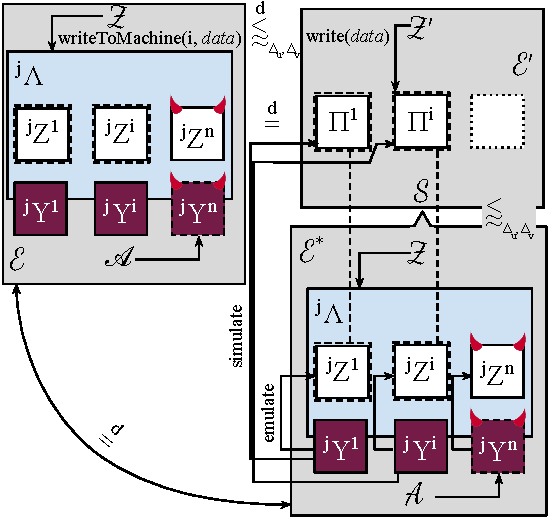
\includegraphics[width=0.7 \textwidth,keepaspectratio]{figures/rollerblade-emulation.pdf}
    \caption{A visualization of the argument that \rollerblade is faithful.
    In the proof of Conjecture~\ref{conj:simulation},
    the simulator $\mathcal{S}$ and simulated environment $\mathcal{Z}'$
    give rise to execution $\mathcal{E}'$ in the
    party setting (top right) by sampling an execution $\mathcal{E}^*$ in the emulated
    setting with adversary $\mathcal{A}$ and environment $\mathcal{Z}$
    (bottom right). The simulator uses each good ledger $\Y[i][j]$ in
    $\mathcal{E}^*$ to feed data into the respective honest party $\PPi[i]$
    in $\mathcal{E}'$. The environments $\mathcal{Z}$ in $\mathcal{E}$ and $\mathcal{Z}'$
    in $\mathcal{E}'$ respectively
    give rise to externalities similar in distribution ($\laterlydistr{\Delta_u,\Delta_v}$,
    middle top),
    whereas the views of the honest parties in $\mathcal{E}$
    and $\mathcal{E}'$ are distributionally equivalent ($\distreq$, middle top).
    The executions $\mathcal{E}$ and $\mathcal{E}^*$ are sampled
    from the same distribution ($\distreq$, bottom left).
    The views of the honest parties in $\mathcal{E}^*$ and $\mathcal{E}'$
    are equal (not just equal in distribution)
    and the externalities in $\mathcal{E}^*$ and $\mathcal{E}'$
    similar (not just similar in distribution).}
    \label{fig.conj.simulation}
  \end{figure*}

  % TODO: consider moving the simulation to an algorithm/figure
  The simulator initially obtains, for every $i \in [n]$,
  a copy of the configuration $M_i$ of the ITI $\RB[j]$ from $\mathcal{E}^*$ at the end of
  $\mathcal{E}^*$.
  The simulator calls $\prepareSimulationInputs(i, \simulationRound, \realityRound)$ on $M_i$
  \emph{in vitro} at the end of round $R$, where $\simulationRound = R - \Delta_v - 1$
  and $\realityRound = R$, to obtain the pair
  $(\writeboxes^i, \inboxes^i)$, where
  $|\writeboxes^i| = R - \Delta_v - 1$
  and
  $|\inboxes^i| = R - \Delta_v - 1$.
  At the beginning of round $r$ of $\mathcal{E}'$, the simulator calls
  $\lwrite(\data)$ on party $i$
  for every $\data \in \writeboxes^i[r - 1]$.
  When $\mathcal{Z}'$ activates party $i$ during round $r$,
  if party $i$ invokes the network receive method $\recv()$, then $\mathcal{Z}'$
  provides $\inboxes^i[r - 1]$.

  % TODO: separate the notion of "emulation" and the notion of "simulation"

  We note that $\mathcal{S}$ uses the adversary $\mathcal{A}$ and the
  environment $\mathcal{Z}$ in this simulation, so $\mathcal{E}$
  and $\mathcal{E}^*$ are identically distributed.
  For (1) it suffices to show that for all $j$,
  $\LCView_{j,H,\Delta_v}(\mathcal{E}^*) = \PEView_H(\mathcal{E}')$
  (i.e., we will show the these two random variables are equal,
  not just equal by distribution),
  and similarly for (2) it suffices to show that for all $j$,
  $\LCExtern_j(\mathcal{E}^*) \laterly{\Delta_u,\Delta_v} \PEExtern(\mathcal{E}')$
  (i.e., we will show that the externalities of $\mathcal{E}'$ are
  similar to $\mathcal{E}^*$, not just \emph{distributionally} similar).

  Since $\mathcal{Z}$ is $B$-respecting, therefore $B(\mathcal{E}^*)$ holds.
  Hence, for all $i \in H$, $\Y[][i]$ is safe, live $(u_i)$, and timely $(v_i)$
  in $\mathcal{E}^*$.

  \noindent
  \textbf{Claim 0: $\mathcal{Z}'$ respects the network model.}
  Namely, the claim is that for all $i, i' \in H$, for all rounds $r$ of $\mathcal{E}'$:

  \begin{enumerate}[label=(\alph*)]
    \item
    \label{conj:simulation:claim-delta}
    If $\PPi[i]$ sends a message to $\PPi[i']$ at round $r$, then this message is delivered to $\PPi[i']$ (with source $i$) by round $r + \Delta$, and

    \item
    If $\PPi[i']$ received a message from $\PPi[i]$ at round $r$, then this message was sent by $\PPi[i]$.
  \end{enumerate}

  If $\PPi[i]$ sends a message $\msg$ to $\PPi[i']$ at round $r$, then
  if we call in vitro (after round $r + \Delta_v$) $\simulate(i, \Ledger[j][i][r], r)$
  on $\LLambda[j]$ we will find that message in $\outboxes[r]$.
  %TODO: prove the above

  At round $r$, relayer $\LLambda[j]$ invokes $\relay()$.
  This creates a transcription $\tau = \Y[j][i].\transcribe()$, where
  $\Y[j][i].\untranscribe(\tau) = \Ledger[j][i][r]$.
  Then, it transmits a new bulletin `checkpoint'
  transaction $\tx$ containing transcription $\tau$ to $\Y[][i']$.

  Because of the liveness of $\Y[][i']$,
  transaction $\tx$ appears in $\Ledger[j][i'][r']$
  at round $r' \leq r + u_{i'} \leq r + \Delta_u$.

  Then, $(\tx, r^*) \in \Ledger[j][i'][R']$. If we call in vitro
  (after round $r + \Delta_v$) $\simulate(i, \Ledger[j][i][r], r)$
  on $\LLambda[j]$ we will find $\msg$ in $\outboxes[r]$.

  That means that when the simulator calls in vitro
  (at the end of round $R$ where $R \geq r' + \Delta_v$) $\prepareSimulationInputs(i', \Ledger[j][i'][R], R - \Delta_v - 1)$
  we will find $m$ in $\inboxes[r^*]$ (with source $i$).
  Therefore, $\mathcal{Z}'$ will provide $m$ to $\PPi[i']$
  if $\PPi[i']$ calls method $\recv()$ at round $r*$.
  %TODO: formalize the above

  This completes the proof of \ref{conj:simulation:claim-delta}.

  %TODO: prove 0b.

  \noindent
  \textbf{Claim 1: $\LCView_{j,H,\Delta_v}(\mathcal{E}^*) = \PEView_H(\mathcal{E}')$.}
  Let $V^* = \LCView_{j,H,\Delta_v}(\mathcal{E}^*)$ and
  $V' = \PEView_H(\mathcal{E}')$.
  We know that $\mathcal{E}^*$ is $(j, H, \Delta_v)$-consistent
  from Lemma~\ref{lem:consistency}, and so $V^*$
  is well-defined.
  The two views have the same size.
  We need to show
  that the views of all \emph{honest} parties in the two executions are identical.
  Let $i$ be an arbitrary party in $H$.

  Let $c^*(r_1, r_2, r_3)$ denote the configuration
  of the machine $\Z[j][i]$ after the invocation of
  Algorithm~\ref{alg.simulate} Line~\ref{alg.simulate:execute}
  during the $r_3$-rd iteration of the \emph{for loop} in
  Algorithm~\ref{alg.simulate} Line~\ref{alg.simulate:for}
  (or, if $r_3 = 0$, we set $c^*(r_1, r_2, r_3)$ to be the state of
  $\Z[j][i]$ before the \emph{for loop})
  when $\emulateMachine$ is
  invoked \emph{in vitro} after round $r_1$ of execution $\mathcal{E}^*$,
  where $r_2 + \Delta_v + 1 \leq r_1 \leq R + \Delta_v + 1$ with parameter
  $\simulationRound = r_2$, and $r_3 \leq r_2$.
  This causes an invocation of \simulate with parameters
  $\simulationRound = r_2$ and $\realityRound = r_1$.
  Let $c'(r_3)$ denote the configuration of the machine $\PPi[i]$
  in $\mathcal{E}'$ at the end of round $r_3$.
  We set $c'(0)$ to be the initial configuration of $\PPi[i]$,
  after it's \emph{constructor} is invoked.

  We will prove that $V^*_{i,r} = V'_{i,r}$ by induction on $r$.
  Let $r$ be an arbitrary round such that $1 \leq r \leq R - \Delta_v - 1$.

  If $r = 1$, then
  \begin{equation}\label{conj:simulation:ind-hyp}
    c^*(r + \Delta_v, r - 1, r - 1) = c'(r - 1)\,
  \end{equation}
  because the state of machine $\Z[j][i]$ and $\PPi[i]$ are identical
  after the initial invocation of the \emph{constructor} as $\Pi$
  is deterministic.

  If $r > 1$, then by inductive hypothesis we have $V^*_{i,r - 1} = V'_{i,r - 1}$
  by which Eq~\ref{conj:simulation:ind-hyp} also follows.

  In either case, Eq~\ref{conj:simulation:ind-hyp} holds, and we
  wish to show that $c^*(r + \Delta_v + 1, r, r) = c'(r)$,
  from which it will follow that $V^*_{i,r} = V'_{i,r}$.

  %TODO: check that induction base holds
  Because $\mathcal{E}^*$ is consistent, we have that
  \begin{equation}\label{conj:simulation:consistency}
    c^*(r + \Delta_v, r - 1, r - 1) = c^*(r + \Delta_v + 1, r - 1, r - 1)\,.
  \end{equation}
  Each iteration of the \emph{for} loop of Algorithm~\ref{alg.simulate} Line~\ref{alg.simulate:for}
  proceeds until the round reaches $\simulationRound$, therefore
  $c^*(r + \Delta_v + 1, r, r - 1) = c^*(r + \Delta_v + 1, r - 1, r - 1)$.
  From this and Eq~\ref{conj:simulation:consistency} we conclude that
  $c^*(r + \Delta_v + 1, r, r - 1) = c^*(r + \Delta_v, r - 1, r - 1)$.
  From this and Eq~\ref{conj:simulation:ind-hyp} we conclude that
  \begin{equation}\label{conj:simulation:pre-state}
    c^*(r + \Delta_v + 1, r, r - 1) = c'(r - 1)\,.
  \end{equation}

  Let $(\writeboxes^*, \inboxes^*)$
  be the pair
  returned by the invocation of $\prepareSimulationInputs(i, \Ledger[j][i][r + \Delta_v + 1], r)$
  \emph{in vitro} after round $r + \Delta_v + 1$ for party $\LLambda[j]$ of $\mathcal{E}^*$, and, likewise define
  $(\writeboxes', \inboxes')$ to be the pair
  returned by the invocation of $\prepareSimulationInputs(i, \Ledger[j][i][R], R - \Delta_v - 1)$
  \emph{in vitro} after round $R$ of $\mathcal{E}^*$ on party $\LLambda[j]$.
  Because $\Y[j][i]$ in $\mathcal{E}^*$ is \emph{sticky} and \emph{timely}$(v_i)$
  the transactions in
  $\Ledger[j][i][r + \Delta_v + 1]$ with recorded round $r - 1$ are identical to
  the transactions in $\Ledger[j][i][R]$ with recorded round $r - 1$
  (all transactions with recorded round $r - 1$ of $\Ledger[j][i][r + \Delta_v + 1]$
   will appear in $\Ledger[j][i][R]$ by stickiness;
   and all transactions with recorded round $r - 1$ of $\Ledger[j][i][R]$ will
   have appeared in $\Ledger[j][i][r + \Delta_v + 1]$ by timeliness; in the case of
   $r = 1$, no transactions with recorded round $r - 1$ will appear in either
   ledger).
  Hence,
  \begin{align}
    \writeboxes^*[r - 1] &= \writeboxes'[r - 1]\label{conj:simulation:eq-inputs-writes}\\
    \inboxes^*[r - 1] &= \inboxes'[r - 1]\label{conj:simulation:eq-inputs-inboxes}\,,
  \end{align}
  since the loop of Algorithm~\ref{alg.prepare-simulation-inputs} Line~\ref{alg.prepare-simulation-inputs:for}
  will run identically in the two invocations of $\prepareSimulationInputs$ up to
  and including round $r - 1$ (and for
  $r = 1$, $\writeboxes^*[0] = \inboxes^*[0] = \writeboxes'[0] = \inboxes'[0]$ by construction).

  By the \rollerblade construction,
  $c^*(r + \Delta_v + 1, r, r)$ is the result of
  taking the machine configuration
  $c^*(r + \Delta_v + 1, r, r - 1)$
  and running the \emph{for} loop of Algorithm~\ref{alg.simulate} Line~\ref{alg.simulate:for}
  for one more iteration, providing inputs $\writeboxes^*[r - 1], \inboxes^*[r - 1]$
  during the execution of $\Z[j][i]$.
  To see why $\writeboxes^*, \inboxes^*$ in particular are used in this iteration,
  note that these correspond to the invocation of $\prepareSimulationInputs$ in
  Algorithm~\ref{alg.simulate} Line~\ref{alg.simulate:recursion}.

  Similarly, by the simulator construction, % TODO: when does the simulator obtain \writeboxes, \inboxes? In vitro R...
  the simulator evolves the machine $\PPi[i]$ in $\mathcal{E}'$ from round $r - 1$,
  in which it has configuration $c'(r - 1)$,
  to round $r$,
  in which it has configuration $c'(r)$,
  by feeding it the inputs $\writeboxes'[r - 1], \inboxes'[r - 1]$.

  As $c^*(r + \Delta_v + 1, r, r - 1) = c'(r - 1)$ (by Eq~\ref{conj:simulation:pre-state})
  and the two configurations evolve using the same inputs (by
  Eqs~\ref{conj:simulation:eq-inputs-writes} and \ref{conj:simulation:eq-inputs-inboxes}),
  and, since $\Pi$ is deterministic,
  therefore $c^*(r + \Delta_v + 1, r, r) = c'(r)$ (see Figure~\ref{fig.emulation-claim-1-induction}).
  We conclude that $V^*_{i,r} = V'_{i,r}$, completing the induction
  and the proof of Claim 1.

  \begin{figure*}
    \centering
    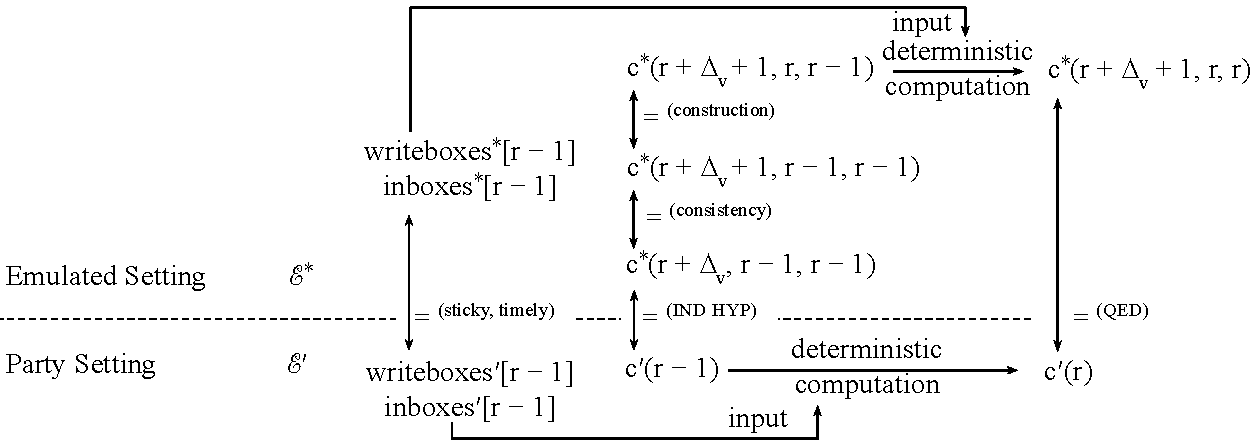
\includegraphics[width=\textwidth,keepaspectratio]{figures/emulation-claim-1-induction.pdf}
    \caption{The inductive step in the proof of the Simulation Conjecture.}
    \label{fig.emulation-claim-1-induction}
  \end{figure*}

  % TODO: double check the exact numbers in this proof

  \noindent
  \textbf{Claim 2: $\LCExtern_{j,H}(\mathcal{E}^*) \laterly{\Delta_u,\Delta_v} \PEExtern(\PEView_{\mathcal{H}(B)}(\mathcal{E}'))$.}

  Let $i \in H$ and $r \leq R - \Delta_u - \Delta_v - 1$ be arbitrary, and $W^i_r$ be the writebox
  at position $(i, r)$ of $\LCExtern(\mathcal{E}^*)$. Let $m$ be an arbitrary message
  in $W^i_r$. Message $m$ was included in a \emph{writeToMachine} call to $\RB[j]$
  with parameter $i$ at round $r$. By the rollerblade construction, the \emph{write}
  function of $\Y[j][i]$ will be called by $\RB[j]$ at round $r$ with parameter a bulletin
  transaction $\tx$ with payload $(\text{`write'}, m)$. Because bulletin transactions are high entropy,
  this transaction is fresh, namely it does not appear in $\Ledger[j][i][r]$.
  Because $i$ is \emph{good}, therefore it is live in $\mathcal{E}^*$ with liveness $u_i$,
  therefore $\tx$ will appear in $\Ledger[j][i][r + u_i]$ with some recorded round $r^*$.
  Note that round $r + u_i \leq R$ falls within the duration of $\mathcal{E}^*$, and
  so the ledger $\Ledger[j][i][r + u_i]$ can be obtained by the simulator.
  Because $i$ is \emph{timely} in $\mathcal{E}^*$ with timeliness $v_i$, therefore
  $r + 1 - \Delta_v \leq r + 1 - v_i \leq r^* \leq r + u_i \leq r + \Delta_u \leq R - \Delta_v - 1$.
  When the function $\prepareSimulationInputs$ is invoked at $\realityRound = R$
  and with $\simulationRound = R - \Delta_v - 1$, the transaction will contribute
  to the \emph{writebox} of party $i$, since $r^* \leq R - \Delta_v - 1$.
  Hence, $m$ will be inputted to the \emph{write} function call of $\Pi^i$
  in $\mathcal{E}'$ at round $r^*$ (and note that $1 \leq r^* \leq R - \Delta_v - 1$ falls
  within the duration of $\mathcal{E}'$), completing the proof of Claim 2.
  \qed
  % TODO: Check that there are sufficient rounds before the end of the simulation
  % for $\Pi^i$ to write this message (i.e., for the message to appear in the prepareSimulationInputs
  % output).
\end{proof}

% TODO: Consider the case of "written communication", or "transferable origin" constructions
% \begin{definition}[Authenticated Communication Protocol]
%       An Authenticated Communication Protocol ACP is...
%       Define what is the syntax of $\Sigma$... (and maybe use a different letter)
%       ... TODO
% \end{definition}
% \begin{definition}[Peer-to-Peer ACP]
%       Make an ACP by composing an existentially unforgeable signature scheme and
%       a synchronous network... TODO
% \end{definition}
% The above definition still allows for use of randomness within the $\Sigma$ protocol of the
% signature, which captures the functionality of generating keys, signing, and verifying
% messages. Typical BFT protocols such as Streamlet~\cite{streamlet} and Hot Stuff~\cite{hotstuff}
% satisfy the \emph{soft determinism} definition.
